%%%%%%%%%%%%%%%%%%%%%%%%%%%%%%%%%%%%%%%%%
% Stylish Article
% LaTeX Template
% Version 2.1 (1/10/15)
%
% This template has been downloaded from:
% http://www.LaTeXTemplates.com
%
% Original author:
% Mathias Legrand (legrand.mathias@gmail.com) 
% With extensive modifications by:
% Vel (vel@latextemplates.com)
%
% License:
% CC BY-NC-SA 3.0 (http://creativecommons.org/licenses/by-nc-sa/3.0/)
%
%%%%%%%%%%%%%%%%%%%%%%%%%%%%%%%%%%%%%%%%%

%----------------------------------------------------------------------------------------
%	PACKAGES AND OTHER DOCUMENT CONFIGURATIONS
%----------------------------------------------------------------------------------------

\documentclass[fleqn,10pt]{SelfArx} % Document font size and equations flushed left

\usepackage[english]{babel} % Specify a different language here - english by default

\usepackage{lipsum} % Required to insert dummy text. To be removed otherwise

%----------------------------------------------------------------------------------------
%	COLUMNS
%----------------------------------------------------------------------------------------

\setlength{\columnsep}{0.55cm} % Distance between the two columns of text
\setlength{\fboxrule}{0.75pt} % Width of the border around the abstract

%----------------------------------------------------------------------------------------
%	COLORS
%----------------------------------------------------------------------------------------

\definecolor{color1}{RGB}{0,0,90} % Color of the article title and sections
\definecolor{color2}{RGB}{0,20,20} % Color of the boxes behind the abstract and headings

%----------------------------------------------------------------------------------------
%	HYPERLINKS
%----------------------------------------------------------------------------------------

\usepackage{hyperref} % Required for hyperlinks
\hypersetup{hidelinks,colorlinks,breaklinks=true,urlcolor=color2,citecolor=color1,linkcolor=color1,bookmarksopen=false,pdftitle={Title},pdfauthor={Author}}

%----------------------------------------------------------------------------------------
%	ARTICLE INFORMATION
%----------------------------------------------------------------------------------------

\JournalInfo{Journal, Vol. XXI, No. 1, 1-5, 2013} % Journal information
\Archive{Additional note} % Additional notes (e.g. copyright, DOI, review/research article)

\PaperTitle{Progress Toward GPU-Accelerated MilkyWay@Home N-Body} % Article title

\Authors{Clayton Rayment} % Authors
% \affiliation{\textsuperscript{1}\textit{Department of Computer Science, Rensselaer Polytechnic Institute}} % Author affiliation

\Keywords{} % Keywords - if you don't want any simply remove all the text between the curly brackets
\newcommand{\keywordname}{Keywords} % Defines the keywords heading name

%----------------------------------------------------------------------------------------
%	ABSTRACT
%----------------------------------------------------------------------------------------

\Abstract{
}

%----------------------------------------------------------------------------------------

\begin{document}

\flushbottom % Makes all text pages the same height

\maketitle % Print the title and abstract box

\tableofcontents % Print the contents section

\thispagestyle{empty} % Removes page numbering from the first page

%----------------------------------------------------------------------------------------
%	ARTICLE CONTENTS
%----------------------------------------------------------------------------------------

\section*{Overview}
This document is an overvew of the GPU N-Body project for MilkyWay@Home, and my contributions to it over the course of my Master's Degree work. As of the writing of this summary, the following has been completed:
\begin{itemize}
    \setlength\itemsep{0.1pt}
    \item Learn OpenCL
    \item Brute Force N-Body Kernels
    \item Bounding Box Kernel
    \item Morton Encoding Kernel
    \item Bitonic Sorting Kernel
    \item Binary Tree Construction Kernel
    \item Naive Parallel Prefix Sum Kernel
    \item Octree Construction Kernel
\end{itemize}
~\\

By the end of the Spring 2018 semester (03/15/2018), the following will be completed:
\begin{itemize}
    \setlength\itemsep{0.1pt}
    \item Full Parallelization of Prefix Sum Kernel
    \item Verify GPU Tree Construction
    \item Octree Threading Kernel
    \item Force Calculation Kernel
    \item Particle Integration Kernel
    \item Result Verification
    \item Error Mitigation
    \item Write Paper
    \item Release on MilkyWay@Home
\end{itemize}
For a more in-depth timeline, please refer to the Remaining Work section.

\section*{Introduction} % The \section*{} command stops section numbering
MilkyWay@Home is a massively distributed computing project which runs on the BOINC network. Users donate computing time to the project, and part of that computing time goes towards simulating the tidal disruption of a dwarf galaxy as it falls into a gravitational potential model of the Milky Way galaxy. Right now, N-Body calculations are all done on the CPU. While some optimization is possible by using a Barnes-Hut treecode algorithm, there is a vast untapped potential for using volunteer GPU time. By porting MilkyWay@Home N-Body to run on users' GPU, we can more efficiently use the volunteer computing time, and allow the userbase to make a larger impact.

The overarching goal of this project is to implement a fully-parallelized GPU Barnes-Hut treecode algorithm on the GPU, which will require no host machine interaction other than periodic checkpointing and release of the GPU to satisfy operating system requirements for GPU utilization. Towards this end, we have written an "exact" N-Body algorithm which computes forces between all particles in the simulation, regardless of distance in relation to the current particle in parallel. Continued work is being done on the "treecode" algorithm, and is detailed in this paper, along with information about the "exact" algorithm.
%------------------------------------------------

\section{OpenCL}
Learned how to use the OpenCL API for accessing the GPU. While using CUDA would be easier, since MilkyWay@Home runs on volunteer computers with unknown hardware, the possiblity of users having AMD/ATI hardware exists, so we use OpenCL to access both NVIDIA and AMD/ATI hardware. OpenCL requires the explicit creation of GPU context information, where the machine is queried for what hardware it contains. Creation of buffers on the GPU for global device memory is done from the host machine once OpenCL is aware of what hardware it is using. To be able to support multiple device architectures, OpenCL kernel code is compiled JIT (Just In Time) when the user runs our OpenCL application. Finally once kernels are created, and buffers allocated, the relevent data is pushed to the GPU, and the simulation is started by pushing kernel calls to the OpenCL command queue. In the future, checkpointing will be addded every few hundred cycles of kernel calls in order to free up the GPU every so often to satisfy OS requirements for GPU utilization, as well as to protect against unexpected shutdown of the application.

%------------------------------------------------

\section{Brute-Force Exact N-Body}
The brute force GPU algorithm is an $O\left(\frac{n^2}{p}\right)$ algorithm where $n$ is the number of particles in the simulation, and $p$ is the number of threads. The algorithm computes forces between each particle exacted by all other particles in the system. This is an extremely slow method, however it does produce the most “exact” results with the least approximation error. In the MilkyWay@Home CPU code, we implement this as well as a more efficient Barnes-Hut treecode. A flow chart of the GPU Exact computation strategy can be seen in Figure 1.

\subsection{Force Calculation Kernels}
The force calculation kernels are relatively simple compared to the other kernels. During each step of the simulation, each particle is assigned to a different thread. To compute the force on the thread's assigned particles, it looks at each particle in the simulation, and computes the distance to that particle, and then using the standard $\frac{1}{r^2}$ gravitational formula, it computes an acceleration on the particle. Floating point error is accumulated the same for each particle, as the list of particles is traversed in the same order by all threads.

\subsection{Integration Kernels}
Integration kernels are broken up into "half action" kernels to match their CPU counterparts. During a step of the simulation, the particle integration sequence is as follows:
\begin{enumerate}
    \setlength\itemsep{0.1pt}
    \item Half velocity update
    \item Position update
    \item Half velocity update
    \item Acceleration calculation
\end{enumerate}
We break the integration up into four interleaved steps in order to get a more precise estimate during the motion. For our purposes, we assume acceleration is constant through the entirety of the motion, which in actuality is not true. While the change in acceleration across the particle's motion, especially with a small simulation timestep, is quite small, by integrating the particle motion in this manner, we help to reduce the error this introduces.

\begin{figure}[h]
    \centering
    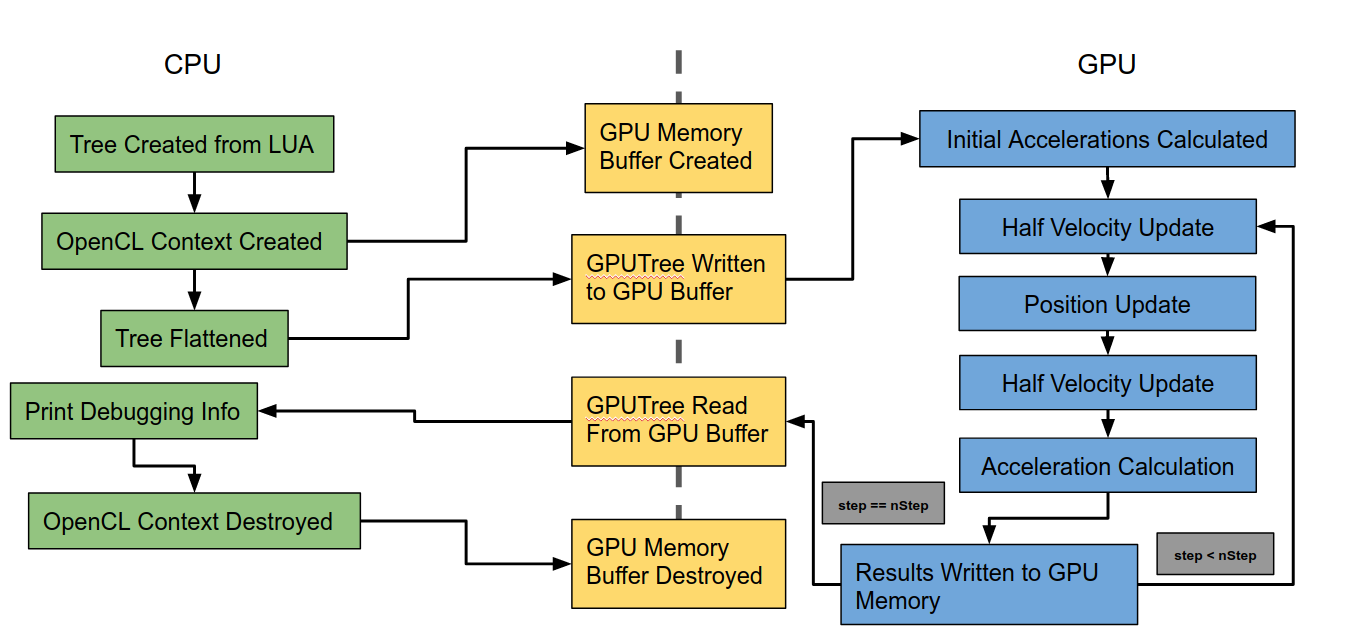
\includegraphics[width=0.5\textwidth]{GPUExact.png}
    \caption{Flow chart of the Exact GPU N-Body algorithm}
\end{figure}



\subsection{Branch Optimization}
Branch divergence on the GPU incurs a significant performance penalty, as groups of processing cores on the GPU operate in lock-step with eachother. Branching within a workgroup causes processors that did not take the branch to perform instruction repetition in order to “wait” for the branched processes to catch up. For example, on current NVIDIA architectures, one thread which diverges from the workgroup can de-rail 31 other threads as they wait for the process to finish. To combat this, if possible, branch statements are replaced with logic multipliers on various values so that branch divergence is not possible.

\subsection{Local Work Group Optimization}
By far the fastest memory on the GPU accessable to multiple threads is in local memory. To further speed up calculations, each work unit chunks off a segment of the data, and then stores it in local memory, based on the workgroup’s ID. This is used for the reduction operations, as well as the particle integration for updating velocity and position. Copying to local memory also prevents threads from colliding when trying to access data which exists in global memory. When two or more threads collide while accessing global memory, the operation is serialized with order determined in a FIFO schedule. This can cause a significant performance penalty, especially on pattern based data access.



% -------------------------------------------------------------------------------

\section{Barnes-Hut treecode N-Body}
The Barnes-Hut algorithm for N-Body calculations makes use of an octree for determining which groups of particles will interact by recursively subdividing the simulation space into octants until each octant contains one or zero particles. Each internal node of the octree contains the center of mass of all of the particles which are children of it (including those in other internal nodes). If the center of mass of a particluar node is far enough away from a given particle, then the interactive forces to the particle which is being calculated is done by the center of mass, rather than all the individual children particles. Performing the force calculations in this way results in an $O(\frac{n}{p} log n)$ complexity, which is much better than the brute force algorithm. On the GPU, however, since we are using OpenCL we can not create recursive kernel calls, and this is not great for parallel performance anyway, so we utilize a method outlined in \cite{Karras:2012} in order to construct the GPU Octree in parallel using a z-order space filling curve. The process is outlined in Figure 2.

\subsection{Bounding Box}
Before treecode can begin, we need to know our simulation bounds. Bounding box does a 3 dimensional reduction operation to compute the min and max for each dimension. Almost all branch statements in the kernel have been eliminated by using logical multipliers as described previously. Since the reduction is on randomly ordered data, the possibility for divergence is very high. 

\subsection{Morton Encoding}
Once we have the simulation bounds, we encode each particle with a 30-bit 3d morton code which corresponds to a z-order space filling curve. The code is calculated by expanding the bits of the positional data, and then interleaving them. Encoding the particles in this manner allows us to sort them based on their location along the 1 dimensional space filling curve, which corresponds deterministically to the particle’s 3 dimensional position.

\subsection{Bitonic Sorting}
Encoded particles then are sorted using a parallel bitonic sorting algorithm. Bitonic sorts are excellent for parallelization, as sort operations are independent of one another, and it can be performed in-place which is perfect for the GPU. Bitonic sort is also agnostic of the input data order, meaning sorts will always take the same amount of time.

\subsection{Binary Tree Construction}
Using the sorted morton codes, a binary tree is constructed based off of the work demonstrated in \cite{Karras:2012}. Each thread in parallel examines its assigned morton code, and determines where its children are, based on the sorted morton code list by examining differences in the morton codes starting from the highest order bit.

\subsection{Parallel Prefix Sum}
Each edge in the binary GPU tree then is examined to determine how many octree nodes it will contribute to the final GPU octree. These counts are put into an array in global memory, indexed inline with the node’s location in the binary tree array. Once this is complete, a parallel prefix sum kernel is run, to determine the number of nodes and final data indexing in the octree. 

\subsection{Octree Construction}
Armed with all of this information, we are finally able to construct the octree by examining the parallel prefix sum array, and the binary tree ancestors. Using this, we fill in the morton prefix of each location of the octree, and then decend the tree starting from the root, matching prefixes with the leaf nodes in order to link them with the internal nodes.

\begin{figure}[h]
    \centering
    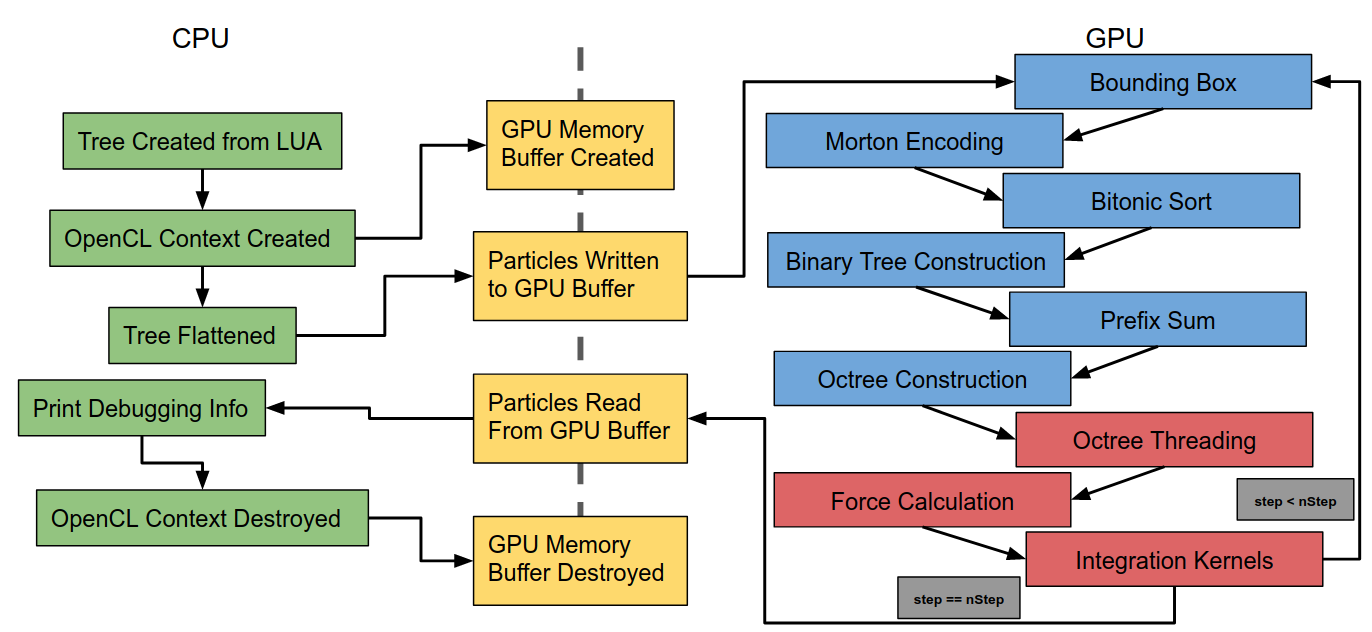
\includegraphics[width=0.5\textwidth]{GPUTreecode.png}
    \caption{Flow chart of the Treecode GPU N-Body algorithm. Kernels that are complete are blue, whereas kernels that remain to be written are red.}
\end{figure}



%------------------------------------------------

\section{Remaining Work}

\subsection{Full Parallelization of Prefix Sum Kernel}
\textbf{EXPECTED COMPLETION: 01/18/2017}\\
Currently the Prefix Sum kernel contributes a large amount to the computation profile. This can be reduced to a very small profile by instead doing an in-place prefix tree reduction. The current computation is done by doing a serial prefix sum for each element of the array in parallel. While this produces a correct result, it is very slow.

\subsection{Verify GPU Tree Construction}
\textbf{EXPECTED COMPLETION: 02/01/2017}\\
Once GPU tree construction is in a state which is stable, sample runs need to be compared to the actual data to see if the hierarchy is generated correctly, and any issues with this need to be debugged before the calculation can continue. Since the hierarchy is what determines what groups of particles get used by the force calculation, small discrepencies in this can cause a huge difference in the way calculations are made.

\subsection{Thread Octree for Force Calculation}
\textbf{EXPECTED COMPLETION: 02/01/2017}\\
To reduce the search times, the simulation octree is threaded with "next" and "more" index pointers which are used during the force calculation to traverse the tree. 


\subsection{Force Calculation}
\textbf{EXPECTED COMPLETION: 02/15/2017}\\
Once the tree is threaded, each processing thread will start at a particle, and calculate all the forces acting on the particle, based on the locations of groups of particles in the octree. If the center of mass of the octree is far enough away, the CoM is treated as a particle, and will be used to compute the interactive forces on the particle of interest.

\subsection{Particle Integration}
\textbf{EXPECTED COMPLETION: 02/15/2018}\\
Following force calculation, the particles must be integrated to find the new velocity and and position after each step of the simulation. This is a simple calculation, and will not add much to the profile, since the interactive force has already been computed. The kernels for this will also be simple, as all the data will be inline, and thread collisions are not an issue, as there is no cross-particle data for this step.

\subsection{Result Verification}
\textbf{EXPECTED COMPLETION: 02/22/2018}\\
Once a simulation is running, the results have to be verified in comparison to the CPU. There will be small differences due to a difference in accumulation of floating point error, but in general the simulations should run the same. Small errors that can not be mitigated such as floating point error will have to be dealt with in the error mitigation section.

\subsection{Error Mitigation}
\textbf{EXPECTED COMPLETION: 03/01/2018}\\
Finally, small errors that will accumulate due to intrinsic differences between CPU and GPU operation will have to be dealt with statistically. This is vitally important as we will be running on a heterogeneous computing platform, with all different types of hardware, and we still need to be able to verify results that get returned from our volunteers, even if the computer that does the result verification is doing it on different hardware.

\subsection{Master's Thesis}
\textbf{EXPECTED COMPLETION: 03/15/2018}\\
A comprehensive paper on this subject will be written, and submitted to OGE as a master's thesis. A committee has already been formed, and the background of the paper is written. As the semester goes on, more will be added to the paper alongside the work done to the code, so the time between 03/01/2018 and 03/15/2018 will be used for addition of graphs, results, and final edits before review with advisors.

\subsection{Release on MilkyWay@Home}
\textbf{EXPECTED COMPLETION: 04/01/2018}\\
All of this code, along with the paper, will be released on MilkyWay@Home, ready for users to start performing GPU N-Body computations for the project. A post on the MilkyWay@Home forums will be made, with a reference to the paper (once approved), so that users can better understand the GPU N-Body code that they will be running.

% ------------------------------------------------
\phantomsection
\section*{Acknowledgments} % The \section*{} command stops section numbering

\addcontentsline{toc}{section}{Acknowledgments} % Adds this section to the table of contents

GPU Binary Tree and GPU Octree construction is done following algorithms presented in \cite{Karras:2012}.

%----------------------------------------------------------------------------------------
%	REFERENCE LIST
%----------------------------------------------------------------------------------------
\phantomsection
\bibliographystyle{unsrt}
\bibliography{sample}

%----------------------------------------------------------------------------------------

\end{document}